\documentclass[conference]{IEEEtran}
\usepackage{amsmath}
\usepackage{newtxtext,newtxmath}
\usepackage{graphicx}
\usepackage{booktabs}
\usepackage{multirow}
\usepackage{xcolor}
\usepackage[hidelinks]{hyperref}
\graphicspath{{../../../results/01-cage/}}

% Every number in this file comes from results/01-cage/**/summary.md (rule E5).
% All of them are scenario values: synthetic workloads + analytic cost model (rule E1).

\begin{document}

\title{CAGE: When Does Communication-Graph\\Structure Pay Off for Rank Placement?}

\author{
\IEEEauthorblockN{Divyansh Verma, Aniruddha Badhani, Ashutosh Singh}
\IEEEauthorblockA{Dept.\ of Computer Science,
Noida Institute of Engineering and Technology, Greater Noida, India\\
\{0241cs202, 0241cs161, 0241cs203\}@niet.co.in}
}

\maketitle

\begin{abstract}
Placing communicating processes close together is a decades-old idea, but whether the
communication graphs of modern distributed training jobs hold structure that a placement can
exploit, beyond what the launcher's rank order already captures, has rarely been tested with
statistical care. We present CAGE, a pipeline that turns communication traces into traffic
graphs, expands collectives by the algorithm that ran, tests community structure against a
degree-preserving null model, and recommends exact-capacity placements. Placements are scored
under two regimes: collectives held in rank order (MPI-like) and collectives re-ringed for each
placement (NCCL-like). On models of data-parallel, Megatron 3D-parallel, mixture-of-experts (MoE)
and stencil workloads, three results stand out. First, raw modularity misleads: a 64-rank ring
scores $Q=0.74$ with $z=-1.1$ against its null model. Second, against block placement, graph-aware
placement gains nothing for data-parallel and default-order Megatron jobs. It gains only where rank
order disagrees with structure: $-93\%$ cross-host bytes for scrambled Megatron ranks, $-43\%$ and
$-25\%$ for 2D and 3D stencils, and $-56\%$ for MoE with routing affinity 0.6, falling to zero
without affinity. Third, a bytes-only graph cannot find a slow NIC (hit rate 0.12, chance 0.125),
while a time-weighted graph does (0.75--1.00). All numbers are scenario values from synthetic
workloads and an analytic bandwidth model, not hardware measurements; we state what real traces
must show to confirm them.
\end{abstract}

\begin{IEEEkeywords}
communication graphs, process placement, graph partitioning, modularity, null models,
distributed training, NCCL, MPI
\end{IEEEkeywords}

% ---------------------------------------------------------------------------------------------
\section{Introduction}

Distributed training jobs spend a large share of each step moving data between accelerators.
When two heavily communicating ranks sit on different hosts, their traffic crosses the network
interface instead of the much faster intra-host links. The idea that a scheduler should place
processes using their communication pattern goes back to Bokhari's mapping
problem~\cite{bokhari1981mapping} and is the basis of tools such as MPIPP~\cite{chen2006mpipp},
TreeMatch~\cite{jeannot2014treematch}, Scotch~\cite{pellegrini1996scotch} and generic topology
mapping~\cite{hoefler2011generic}; MPI even standardises rank reordering from a declared
graph~\cite{traff2002topology,mpi40}. We therefore do \emph{not} claim that building a
communication graph and partitioning it is new.

What is missing is an honest answer to a narrower question: \emph{for the communication patterns
of modern training jobs, when does graph-aware placement beat the placement a launcher already
produces?} Three pitfalls make the obvious experiment misleading. (i) Modularity is high for
graphs with no community structure at all, such as rings and sparse random
graphs~\cite{guimera2004modularity}, so a fixed threshold such as ``$Q>0.3$'' reports structure that
is not there. (ii) Round-robin placement is a strawman; the realistic default is \emph{block}
placement (SLURM block, \texttt{torchrun}), which already co-locates consecutive ranks.
(iii) Libraries such as NCCL rebuild ring order from the detected topology, so traffic of a
collective expanded in the original rank order is not fixed when ranks move.

CAGE is built around these pitfalls. Our contributions are:
\begin{enumerate}
\item A trace-to-placement pipeline that expands collectives by the algorithm that ran, keeps
      per-step and per-operation detail, and scores placements in two regimes: collectives
      fixed in rank order, and collectives re-ringed for each candidate placement
      (Section~\ref{sec:design}).
\item A null-model protocol for community structure (degree-preserving rewiring, $\geq 19$
      samples, $z>3$, $p\leq 0.05$) and exact-capacity partitioning that is never worse than
      block placement by construction.
\item An empirical characterisation across data-parallel, Megatron 3D-parallel, MoE and stencil
      workloads that includes negative results, a simple decision rule for when placement pays,
      and evidence that bytes-only graphs cannot locate time bottlenecks (Section~\ref{sec:results}).
\end{enumerate}

\textbf{Scope of evidence.} Every workload in this paper is a synthetic model with known ground
truth, and every time is the output of an analytic bandwidth model. We call these numbers
\emph{scenario values}. They rank placements; they do not predict wall-clock speedups.
Section~\ref{sec:threats} lists what real traces must confirm.

% ---------------------------------------------------------------------------------------------
\section{Background and Related Work}\label{sec:related}

\textbf{Topology and process mapping.} Mapping a task graph onto a machine graph is NP-hard in
general~\cite{bokhari1981mapping}. Practical tools extract a communication matrix and partition
it: MPIPP profiles MPI programs and places processes on SMP clusters~\cite{chen2006mpipp};
TreeMatch maps onto hierarchical machines~\cite{jeannot2014treematch}; Scotch performs dual
recursive bipartitioning of process and architecture graphs~\cite{pellegrini1996scotch};
Hoefler and Snir compare generic mapping heuristics~\cite{hoefler2011generic}. A survey is given
in~\cite{hoefler2014overview}. CAGE uses the same core machinery (METIS~\cite{karypis1998metis} and
Kernighan--Lin-style refinement~\cite{kernighan1970}). Our contribution is the measurement
protocol and the characterisation, not the partitioner.

\textbf{Communication analysis tools.} Score-P and Vampir show communication
matrices~\cite{knupfer2012scorep}; Chakra standardises execution traces for ML
workloads~\cite{sridharan2023chakra}; ScalAna applies graph analysis to locate scaling
loss~\cite{jin2020scalana}. These tools visualise or diagnose; they do not ask when a
placement change would help relative to the launcher default.

\textbf{ML communication.} Data parallelism uses ring or hierarchical
allreduce~\cite{sergeev2018horovod,thakur2005mpich,patarasuk2009bandwidth}; Megatron-LM combines
tensor, pipeline and data parallelism with a fixed rank order~\cite{shoeybi2019megatron,
narayanan2021megatron}; MoE models add all-to-all token routing~\cite{lepikhin2021gshard,
fedus2022switch}, and FasterMoE exploits topology in expert placement~\cite{he2022fastermoe}.
ByteScheduler~\cite{peng2019bytescheduler} schedules communication and
TopoOpt~\cite{wang2023topoopt} co-designs topology with parallelisation. CAGE is complementary:
it asks whether the traffic graph itself says that ranks are in the wrong place.

\textbf{Community structure and null models.} Modularity~\cite{newman2004finding} optimised by
Louvain~\cite{blondel2008louvain} finds communities but is biased: random and regular graphs reach
high $Q$~\cite{guimera2004modularity}, and modularity has a resolution
limit~\cite{fortunato2007resolution}. Degree-preserving rewiring~\cite{maslov2002specificity} gives
the standard null model; we use it for every reported $Q$.

% ---------------------------------------------------------------------------------------------
\section{CAGE Design}\label{sec:design}

\subsection{Trace model}
A trace is an event table, not a graph. Each event records source rank, destination rank,
bytes, message count, step index, operation name and, when the source provides it, duration.
The static traffic matrix $M$ ($M_{ij}$ = bytes from $i$ to $j$), per-step matrices and arbitrary
windows are views of the same table. The undirected view is $W=M+M^\top$. Keeping steps lets the
same data serve a static analysis (this paper) and iteration-level analysis (future work).

\subsection{Collective expansion}
A collective is expanded into the point-to-point transfers of the algorithm that ran, because
that is what the network carries. For a ring allreduce of $S$ bytes over $p$ ranks each ring edge
carries $2(p-1)S/p$; for ring allgather and reduce-scatter, $(p-1)S/p$; chain broadcast and reduce
carry $S$ per edge; all-to-all carries the routed bytes directly~\cite{thakur2005mpich,
patarasuk2009bandwidth}. Hierarchical variants (leader-based~\cite{sergeev2018horovod} and
rail-based) are compositions of these. The operation name is kept on every event, so a different
expansion can replace the assumed one without re-collecting traces. Each recorded library
collective is also stored with its member list, so it can be re-expanded for a new placement.

\subsection{Load and hotspot metrics}
The strength (weighted degree) of rank $i$ is $s_i = \sum_j W_{ij}$, so $\sum_i s_i = 2\sum_{ij}M_{ij}$:
each byte has a sender and a receiver. A unit test enforces this identity. We report load
concentration as the Gini coefficient of $s$ and the share of total strength held by the busiest
20\% of ranks. Hotspots are ranks whose robust $z$-score (median and scaled MAD) exceeds 3.5;
the robust score avoids masking by a few large hubs.

\subsection{Community structure with a null model}
We run Louvain on $W$ and compare its modularity $Q$ with $N$ null graphs drawn by
degree-preserving double-edge swaps that carry edge weights~\cite{maslov2002specificity} (weight
shuffling for graphs denser than 80\%). We report
\begin{equation}
z = \frac{Q-\overline{Q}_{\mathrm{null}}}{\sigma_{\mathrm{null}}},\qquad
p = \frac{1+\#\{Q_{\mathrm{null}}\geq Q\}}{1+N},
\end{equation}
and call structure \emph{significant} only if $N\geq 19$, $z>3$ and $p\leq 0.05$. With $N=20$ the
smallest attainable $p$ is $1/21\approx0.048$.

\subsection{Exact-capacity placement}
Hosts have a fixed number of accelerator slots $g$ (8 here), so a placement must put exactly $g$
ranks on each host. METIS only bounds imbalance, so we run it with the tightest imbalance factor,
repair overfull parts greedily (moving the rank that loses the least cut), and then apply
best-improvement pairwise swaps whose gain for $i\in a$, $j\in b$ is
\begin{equation}
\Delta_{ij} = D_{ib}-D_{ia}+D_{ja}-D_{jb}-2W_{ij},
\end{equation}
where $D_{ip}$ is the weight from $i$ to part $p$. Swaps keep capacity exact. The recommended
placement is the lowest-cut result of three seeds (METIS, block, random), so it is never worse than
block placement. Parts are finally renamed by Hungarian matching~\cite{kuhn1955hungarian} so as few
ranks as possible move.

\subsection{Two placement regimes}
\textbf{Fixed.} All traffic, with collectives in their recorded rank order, moves with the
ranks. This is valid for MPI codes whose collective algorithms follow rank order, and for traffic
pinned to rank identity: point-to-point, pipeline sends, halo exchange and expert all-to-all.

\textbf{NCCL.} Rank-pinned traffic moves with the ranks, while every recorded library collective
is re-expanded as a ring ordered by host for each candidate placement, as NCCL derives rings from
the detected topology. The partitioning objective in this regime adds a clique expansion of each
collective (weight $8e/p^2$ per member pair for $e$ ring bytes), which makes an even two-way split
cost the same as the two crossing ring edges it causes. Candidates from both objectives and block
placement are scored under the NCCL model and the best is kept. For GPU jobs this regime is the
headline; the fixed regime overstates what moving ranks can achieve.

\subsection{Cost model}
For host $h$ with egress $E_h$ and ingress $I_h$ cross-host bytes, intra-host bytes $X_h$ and
$m_h$ messages,
\begin{equation}
T_h = \frac{\max(E_h,I_h)}{B_{\mathrm{nic}}f_h} + \frac{X_h}{B_{\mathrm{intra}}} + \alpha\, m_h,
\qquad T = \max_h T_h,
\end{equation}
with $B_{\mathrm{nic}}=50$\,GB/s per direction (400\,Gb/s), $B_{\mathrm{intra}}=300$\,GB/s,
$\alpha=5\,\mu$s and $f_h=1$ unless a fault is injected. The model ignores compute overlap,
dependencies and in-fabric congestion. It ranks placements; it does not predict seconds.

\subsection{Extraction}
CAGE reads its own event CSV, NCCL debug logs (\texttt{NCCL\_DEBUG=INFO},
\texttt{SUBSYS=INIT,COLL}), Chakra execution traces in JSON form~\cite{sridharan2023chakra}, and the
output of a PMPI interposition library that records collectives as collectives, with communicator
membership and durations. PMPI cannot see PyTorch GPU jobs, which call NCCL, not MPI. The parsers
are tested against hand-written fixtures only; validating them on real logs is future work
(Section~\ref{sec:threats}).

% ---------------------------------------------------------------------------------------------
\section{Methodology}\label{sec:method}

\textbf{Workloads.} Table~\ref{tab:workloads} lists the synthetic generators. Rank order follows
each launcher's default (block for data parallel, Megatron's TP-fastest order, MPI Cartesian
row-major order), so the block baseline is realistic. Two perturbations model a mismatch between
rank order and structure: a random relabelling of Megatron ranks (``scrambled''), and MoE data
groups interleaved across ranks ($g(r) = r \bmod 8$) with a routing-affinity knob $a$, the fraction
of a token's routing probability placed on experts hosted inside its own data group. Whether real
MoE training shows rank-level affinity is an open empirical question; $a$ lets us show both sides
of it.

\begin{table}[t]
\caption{Synthetic workloads (all bf16, 8 GPUs per host).}\label{tab:workloads}
\centering\footnotesize
\begin{tabular}{@{}lp{4.9cm}@{}}
\toprule
Workload & Model \\
\midrule
DP ring & flat ring allreduce of 2\,GB gradients per step \\
DP hier.\ leader / rail & Horovod-style leader allreduce / rail-optimised allreduce \\
Megatron TP$\cdot$PP$\cdot$DP & 8$\cdot$4$\cdot$2, $L{=}32$, $h{=}8192$, seq 4096, 8 microbatches; TP ring allreduce, PP sends (scatter-gather), DP allreduce of the parameter shard \\
MoE & EP $=64$ ranks, 2 experts/rank, top-2, Zipf expert popularity (default 1.0), affinity $a$, plus dense 2\,GB ring allreduce \\
Stencil & halo exchange of 4\,MB per face on 8$\times$8 or 4$\times$4$\times$4 grids \\
SBM & planted partition~\cite{holland1983sbm}, 64 ranks in 8 blocks, log-normal weights \\
\bottomrule
\end{tabular}
\end{table}

\textbf{Baselines.} Block placement (ranks $[0,g)$ on host 0, \ldots) is the reference. Round-robin
($r \bmod H$) is shown only beside it. Reductions are $1-x_{\mathrm{CAGE}}/x_{\mathrm{block}}$.

\textbf{Protocol.} Seeds are fixed. Each experiment script states its expected result before it
is run, and misses are reported. Every number in this paper is read from a results file generated
by the published scripts (see Artifact Availability).

% ---------------------------------------------------------------------------------------------
\section{Results}\label{sec:results}

\subsection{Raw modularity is not evidence (E2)}
Table~\ref{tab:null} compares observed Louvain $Q$ with the null-model mean for graphs whose
structure is known. A 64-rank ring has $Q=0.74$ but its null graphs reach $0.76$ ($z=-1.1$); a
sparse random graph of mean degree 4 has $Q=0.48$ ($z=2.1$, $p=0.095$); Horovod-style hierarchical
allreduce has $Q=0.65$ ($z=-0.8$). All three pass the old ``$Q>0.3$'' rule and none has significant
structure. The 2D stencil, the planted partition and Megatron are significant ($z=6.2$, $17.4$ and
$10.2$). MoE without affinity is not ($z=-0.1$).

\begin{table}[t]
\caption{Observed vs.\ null-model modularity, 20 null samples (E2). Scenario values.}\label{tab:null}
\centering\footnotesize
\setlength{\tabcolsep}{3pt}
\begin{tabular}{@{}lrrrrcc@{}}
\toprule
Graph & $Q$ & null $Q$ & $z$ & $p$ & $Q{>}0.3$ & sig. \\
\midrule
ring (64)                  & 0.740 & 0.756 & $-1.1$ & 1.000 & yes & no \\
random sparse, deg 4       & 0.482 & 0.445 & 2.1  & 0.095 & yes & no \\
random dense, deg 32       & 0.080 & 0.089 & $-1.9$ & 0.952 & no  & no \\
complete, uniform          & 0.000 & 0.000 & 0.0  & 1.000 & no  & no \\
hier.\ leader (32)         & 0.653 & 0.677 & $-0.8$ & 0.714 & yes & no \\
MoE, no affinity           & 0.224 & 0.225 & $-0.1$ & 0.571 & no  & no \\
2D stencil 8$\times$8      & 0.594 & 0.500 & 6.2  & 0.048 & yes & yes \\
SBM, $\mu\approx0.15$      & 0.685 & 0.445 & 17.4 & 0.048 & yes & yes \\
Megatron 8$\cdot$4$\cdot$2 & 0.821 & 0.661 & 10.2 & 0.048 & yes & yes \\
\bottomrule
\end{tabular}
\end{table}

\subsection{Recovery of planted structure (E1)}
Planted partitions with mixing $\mu$ (the expected share of a rank's traffic that leaves its block)
are relabelled at random, so rank order carries no hint. Fig.~\ref{fig:e1} shows the mean over five
seeds. Louvain NMI~\cite{danon2005comparing} falls from 0.99 at $\mu=0.05$ to 0.51 at $\mu=0.6$ and
0.27 at $\mu=0.75$; exact-capacity partition ARI~\cite{hubert1985ari} falls from 0.99 to 0.33 and
0.12. Significance tracks recovery: $z$ falls from 25.1 to 3.3 at $\mu=0.6$ and 0.6 at $\mu=0.75$,
so CAGE's detection limit lies between $\mu=0.6$ and $0.75$. Above it, CAGE reports \emph{no
structure} rather than inventing communities.

\begin{figure}[t]
\centering
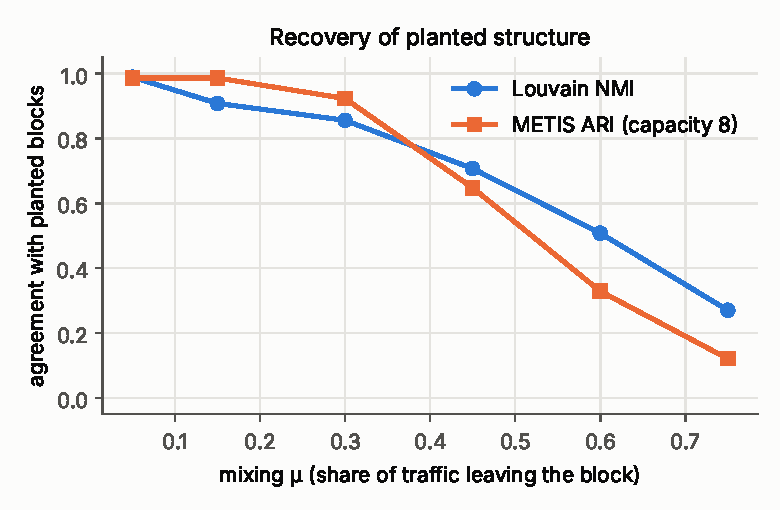
\includegraphics[width=0.49\columnwidth]{e1_synthetic_recovery/recovery_vs_mixing.pdf}\hfill
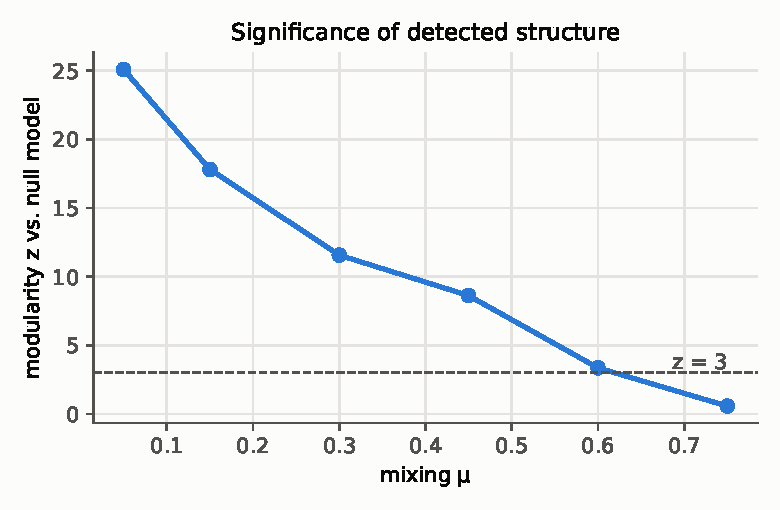
\includegraphics[width=0.49\columnwidth]{e1_synthetic_recovery/z_vs_mixing.pdf}
\caption{E1: recovery of planted blocks (left) and null-model $z$ (right) against mixing $\mu$.
Scenario values.}\label{fig:e1}
\end{figure}

\subsection{Workload characterisation (E3)}
Table~\ref{tab:e3} characterises each workload. The original hypothesis that the busiest 20\% of
ranks carry 70--80\% of traffic fails everywhere: the largest top-20\% share is 0.42 (MoE with Zipf
1.5), and collective-based data parallelism is balanced by design (Gini 0.00 for the flat ring and
rail allreduce, 0.10 for leader-based allreduce, whose leaders carry the inter-host ring). Skewed MoE routing
creates hotspots (6 and 11 ranks above robust $z=3.5$ for Zipf 1.0 and 1.5) but no community
structure; its $Q$ is \emph{below} the null mean at Zipf 1.5 ($z=-5.0$) because a few hub experts
connect everything. Megatron and the stencils are significant. Rail-optimised allreduce is
significant ($z=5.7$) while leader-based allreduce is not ($z=0.0$), yet in both cases the
structure is defined by the algorithm's own host layout: significance alone does not mean a placement
will help, and Section~\ref{sec:e4} shows that, as we test it, it is not required either.

\begin{table}[t]
\caption{Load concentration and structure, 64 ranks, 20 null samples (E3). Scenario values.}\label{tab:e3}
\centering\footnotesize
\begin{tabular}{@{}lrrrrrr@{}}
\toprule
Workload & Gini & top-20\% & hotspots & $Q$ & $z$ & $p$ \\
\midrule
DP ring              & 0.00 & 0.20 & 0  & 0.74 & $-1.1$ & 1.000 \\
DP hier.\ leader     & 0.10 & 0.25 & 0  & 0.75 & 0.0 & 0.381 \\
DP hier.\ rail       & 0.00 & 0.20 & 0  & 0.76 & 5.7 & 0.048 \\
Megatron 8$\cdot$4$\cdot$2 & 0.00 & 0.20 & 0 & 0.82 & 10.2 & 0.048 \\
MoE Zipf 0           & 0.01 & 0.21 & 0  & 0.23 & 2.2 & 0.048 \\
MoE Zipf 1.0         & 0.19 & 0.35 & 6  & 0.22 & $-0.1$ & 0.571 \\
MoE Zipf 1.5         & 0.27 & 0.42 & 11 & 0.22 & $-5.0$ & 1.000 \\
MoE Zipf 1, $a{=}0.6$ & 0.15 & 0.32 & 6 & 0.28 & 2.5 & 0.048 \\
Stencil 2D 8$\times$8 & 0.09 & 0.23 & 0 & 0.59 & 6.2 & 0.048 \\
Stencil 3D 4$\times$4$\times$4 & 0.10 & 0.25 & 0 & 0.54 & 6.8 & 0.048 \\
\bottomrule
\end{tabular}
\end{table}

\subsection{When placement beats block (E4)}\label{sec:e4}
Table~\ref{tab:e4} is the headline. In the NCCL regime CAGE gains nothing for DP ring, hierarchical
DP and Megatron in its default order, and moves no ranks: block placement is already optimal, and
CAGE says so. Megatron is strongly structured ($z=10.2$) but its rank order already matches that
structure. Gains appear only where rank order disagrees with structure: scrambled Megatron ranks
($-92.7\%$ cross-host bytes, $-78.7\%$ modelled time, 48 ranks moved), the 2D and 3D stencils
($-42.9\%$ and $-25.0\%$ bytes, because Cartesian row-major order cuts the grid into thin slabs), and
MoE with routing affinity 0.6 ($-56.3\%$ bytes). Round-robin is catastrophic wherever rank order is
right ($+700\%$ bytes for hierarchical DP, $+1657\%$ for Megatron); the flat DP ring is the
exception only because NCCL re-rings it to the same cost. It ties CAGE on affinity MoE
only because the interleaved data groups ($r \bmod 8$) coincide exactly with round-robin hosts.

For MoE without affinity, cross-host bytes do not change ($-0.1\%$) while modelled time falls by
14.9\%: the partition shifts load between NICs rather than removing traffic. Since the cost model
takes the busiest host, we treat this as a load-balancing side effect, not a structure-driven gain.

\begin{table}[t]
\caption{Placement vs.\ block, 64 ranks (E4). $\Delta$ = change vs.\ block; negative is better.
Scenario values.}\label{tab:e4}
\centering\footnotesize
\setlength{\tabcolsep}{3pt}
\begin{tabular}{@{}lrrrrr@{}}
\toprule
& \multicolumn{3}{c}{NCCL regime, CAGE} & RR & Fixed \\
\cmidrule(lr){2-4}
Workload & $\Delta$bytes & $\Delta$time & moved & $\Delta$bytes & $\Delta$bytes \\
\midrule
DP ring                   & 0.0\%     & 0.0\%     & 0  & 0.0\%      & 0.0\% \\
DP hier.\ leader$^\dagger$ & 0.0\%     & 0.0\%     & 0  & $+700\%$   & 0.0\% \\
Megatron 8$\cdot$4$\cdot$2 & 0.0\%    & 0.0\%     & 0  & $+1657\%$  & 0.0\% \\
Megatron, scrambled       & $-92.7\%$ & $-78.7\%$ & 48 & $-11.1\%$  & $-93.9\%$ \\
Stencil 2D 8$\times$8     & $-42.9\%$ & $-27.3\%$ & 40 & 0.0\%      & $-42.9\%$ \\
Stencil 3D 4$\times$4$\times$4 & $-25.0\%$ & $-31.4\%$ & 32 & $+50.0\%$ & $-25.0\%$ \\
MoE, $a=0$                & $-0.1\%$  & $-14.9\%$ & 46 & 0.0\%      & 0.0\% \\
MoE, $a=0.6$              & $-56.3\%$ & $-48.8\%$ & 56 & $-56.3\%$  & $-13.3\%$ \\
\bottomrule
\multicolumn{6}{@{}p{0.95\columnwidth}@{}}{\scriptsize $^\dagger$The hierarchical generator records no
re-ringable collectives, so its NCCL row equals the fixed regime. RR = round-robin.}
\end{tabular}
\end{table}

\textbf{Fixed vs.\ NCCL regime.} The regimes agree on pinned traffic (stencils) and differ where
collectives dominate. For MoE with $a=0.6$, the fixed regime credits only $-13.3\%$: holding the
dense 2\,GB allreduce ring in rank order makes every placement that departs from rank order pay
for a scattered ring, which NCCL would in practice rebuild.

\textbf{Affinity sweep.} Fig.~\ref{fig:e4sweep} varies affinity. With interleaved groups the gain
grows almost linearly: $-18.8\%$, $-37.5\%$, $-56.3\%$, $-75.1\%$ cross-host bytes at
$a=0.2,0.4,0.6,0.8$. With groups aligned to hosts it is zero at every affinity, because block
placement is already correct. The gain grows in proportion to $a$, so in part it reads back the
generator's parameter. The rule that follows is: \emph{placement pays when the traffic has structure
that disagrees with the launcher's rank order}. Our significance test does not detect that structure
reliably. MoE with $a=0.6$ is not significant on the full graph (Table~\ref{tab:e3}): no null graph
reaches its $Q$ ($p=0.048$, the minimum attainable), but $z=2.5$ falls short of 3. Yet it gains
$-56.3\%$. We suspect the dense allreduce hides the expert structure: once re-ringed it costs the
same for every exact-capacity placement, yet it dominates the graph that Louvain sees. Testing
significance on rank-pinned traffic alone is future work. What decides is the direct comparison:
the recommended partition against block placement under the NCCL model, which is computable from a
trace before anything is moved. The null-model test guards against reporting structure that is not
there; it is not a gate that placement must pass.

\begin{figure}[t]
\centering
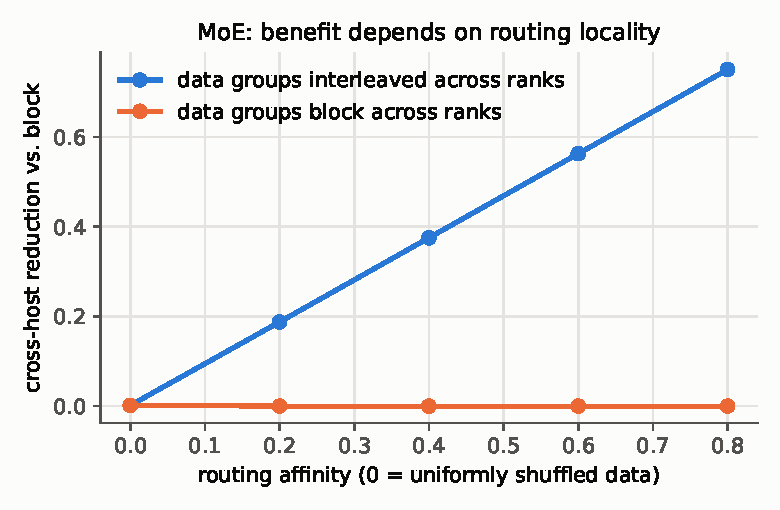
\includegraphics[width=0.85\columnwidth]{e4_placement_benefit/moe_affinity_sweep.pdf}
\caption{E4: MoE cross-host reduction vs.\ block against routing affinity, NCCL regime. Scenario
values.}\label{fig:e4sweep}
\end{figure}

\subsection{Bytes are not bottlenecks (E5)}
Injecting extra bytes and finding them with a bytes metric is circular, so E5 uses two anomalies
(Table~\ref{tab:e5}). Tripling one rank's traffic is found by bytes strength in Megatron (hit rate
1.00) and the stencil (0.97), but only 0.06 of the time in skewed MoE, where hot experts already
dominate strength. The real test runs one host's NIC at 25\% bandwidth, which leaves bytes
unchanged. Bytes strength then picks the slow host at chance (0.12; chance is $1/8$). Time-weighted
strength, with each edge weighted by its transfer time, finds it every time in MoE and Megatron and
0.75 of the time in the stencil. A sanity row confirms that the slowed host is the model's true
bottleneck in every case. Real extraction therefore has to record per-event durations, which
Chakra and the PMPI library do and NCCL INFO logs do not.

\begin{table}[t]
\caption{Anomaly detection, hit rate at rank 1 (E5). Scenario values.}\label{tab:e5}
\centering\footnotesize
\begin{tabular}{@{}lrrr@{}}
\toprule
& volume $\times3$ & \multicolumn{2}{c}{NIC at 25\%} \\
\cmidrule(lr){2-2}\cmidrule(lr){3-4}
Workload & bytes & bytes & time-weighted \\
\midrule
MoE, $a=0$                 & 0.06 & 0.12 & 1.00 \\
Megatron 8$\cdot$4$\cdot$2 & 1.00 & 0.12 & 1.00 \\
Stencil 2D 8$\times$8      & 0.97 & 0.12 & 0.75 \\
\bottomrule
\end{tabular}
\end{table}

\subsection{How much trace is needed (E6)}
A 200-step MoE run ($a=0.6$, doubled routing noise) is sampled every $k$-th step. Placement
quality, defined as the share of the full-trace cut reduction that a placement computed from the
sample retains on the full traffic, stays at 1.000 down to 1\% of steps (2 steps). Community NMI
stays at 1.000, hotspot order (Kendall $\tau$) falls only from 1.000 to 0.945, and top-10 hotspot
overlap drops to 0.818 from 10\% of steps onward. When routing is stationary, a few steps suffice.
Non-stationary routing breaks this, and that is the subject of follow-up work.

\subsection{Overhead (E7)}
On Megatron-style graphs up to 1024 ranks (a laptop with an Intel i5-13420H), load metrics take
0.009\,s, Louvain 0.060\,s, METIS 0.208\,s and sampled betweenness ($k=64$ pivots) 0.252\,s. The
full recommendation with swap refinement takes 0.79\,s at 512 ranks and 10.7\,s at 1024: dense
best-improvement swaps cost $O(n^2)$ per iteration and dominate. Restricting swaps to boundary
vertices or updating gains incrementally is the obvious fix. Timings are machine-dependent.

% ---------------------------------------------------------------------------------------------
\section{Discussion and Threats to Validity}\label{sec:threats}

\textbf{What the results say.} Graph analysis is most useful when it says ``do nothing'': for the
two most common training layouts, data parallelism and Megatron in launcher order, block placement
is already optimal. Its value lies in detecting mismatches: scrambled or heterogeneous launches,
MPI Cartesian codes on GPU hosts, and MoE models whose routing has data-group locality. Each of
these is detectable from a trace by comparing the recommended partition with rank order under the
NCCL model; the significance test prevents false claims of structure but, as the MoE case shows, can
miss real structure.

\textbf{When a trace is not needed.} If the parallelism layout is known (TP, PP, DP and EP group
sizes), a scheduler can place groups by rule, for example each TP group inside one host, without
any trace, and NCCL already orders its rings by topology. Trace-based analysis adds value only where
structure is not visible in the configuration: data-dependent routing, irregular MPI codes,
fragmented allocations, and launches whose rank order silently departs from the intended layout.
Our scrambled-Megatron case is a stand-in for the last; how often it occurs in practice is untested.

\textbf{Synthetic workloads.} Every workload is a model. MoE routing affinity is a parameter, not
an observation; load-balancing losses in real MoE training may suppress it. Megatron is modelled
without sequence parallelism or a distributed optimiser.

\textbf{Collective algorithms.} NCCL chooses ring, tree or NVLS algorithms at run time; INFO-level
logs do not say which ran, so CAGE must assume one and records the assumption. The tree is modelled
as a single binary tree, which overstates per-edge bytes by up to $2\times$ relative to NCCL's
double binary tree. The NCCL regime orders rings by host but does not model NCCL's channel count
or intra-host topology search.

\textbf{Cost model.} The bandwidth model ignores compute overlap, dependencies and congestion inside
the fabric, so modelled time reductions are an upper bound on what a real job would gain from
communication alone.

\textbf{Extraction.} The NCCL, Chakra and PMPI parsers pass tests on hand-written fixtures but have
not yet been run on real logs; the PMPI library has not been compiled against a real MPI. Fortran
codes may bypass a C interposition layer, depending on the MPI implementation's bindings.

\textbf{Betweenness.} Messages in an application-level graph do not travel through intermediate
ranks, so shortest-path centrality has no physical meaning here. CAGE computes it
(with distance $=1/$weight) only as an experimental feature and we draw no conclusions from it.

\textbf{What would confirm the results.} (i) NCCL logs or Chakra traces from real multi-GPU jobs,
to check that data-parallel and Megatron jobs show the predicted ``no gain'' and to measure MoE
routing affinity directly; (ii) MPI traces of the NAS Parallel Benchmarks~\cite{bailey1991nas}
under the PMPI library; (iii) replay of recommended placements in a simulator such as
ASTRA-sim~\cite{rashidi2020astra} or SimGrid~\cite{casanova2014simgrid}, or on a cluster
allocation, to replace the analytic model with measured step times.

% ---------------------------------------------------------------------------------------------
\section{Conclusion}
CAGE turns communication traces into significance-tested graphs and exact-capacity placements
scored under the regime the communication library actually implements. On models of today's
training and HPC workloads it reaches a deliberately modest conclusion: communication-aware
placement beats the launcher default only when the traffic carries structure that disagrees with
rank order. Raw modularity cannot tell structured from unstructured graphs; a null-model test can
guard against false structure but can also miss real structure hidden under placement-neutral
collectives, and a bytes-only graph cannot locate time bottlenecks. Real traces are the next step; the pipeline
and the experiments are ready for them.

\section*{Artifact Availability}\label{sec:artifact}
The code, the seven experiment scripts (E1--E7) and every results file behind this paper's
numbers are available at \url{https://github.com/n0tdivyansh/cage-research}. \texttt{python -m pytest} runs the invariants
the numbers depend on; \texttt{cage run --paper 1} regenerates all results (runtimes are
machine-dependent).

\bibliographystyle{IEEEtran}
\bibliography{refs}

\end{document}
